\documentclass[10.5pt]{article}
\usepackage[margin=2cm]{geometry}
\usepackage[utf8]{inputenc}
\usepackage[T1]{fontenc}
\usepackage{lmodern}
\usepackage{graphicx}
\usepackage{booktabs}
\usepackage{array}
\usepackage{xcolor}
\usepackage[hidelinks]{hyperref}
\setlength{\parindent}{0pt}
\setlength{\parskip}{4pt}
\definecolor{acento}{HTML}{0e7a72}
\definecolor{riesgo}{HTML}{a63d3d}
\pagestyle{plain}

\begin{document}

\begin{center}
{\LARGE \bfseries Monitoreo transaccional: \\[2pt] ¿el orden de las transacciones vale la pena?}\\[6pt]
{\large Informe para el comité de riesgos — Banco del Altiplano}\\[2pt]
\small Luis Pedro Lira · Mario Rocha \quad|\quad Universidad del Valle, Deep Learning 2026
\end{center}

\vspace{2pt}
\textbf{Pregunta del comité:} ¿el orden de las transacciones de una tarjeta aporta información que
las variables agregadas actuales (monto promedio 24h, transacciones por hora, monto máximo del día,
diversidad de comercios) no capturan, y cuánto vale esa información en quetzales? Este informe
responde con evidencia, no con una recomendación de arquitectura.

\textbf{Resumen ejecutivo:} sí aporta. Un modelo que lee la secuencia de eventos (Modelo B) separa
mejor el fraude que el modelo actual basado solo en agregados (Modelo A), y cuando se destruye
artificialmente el orden de esos mismos eventos, el desempeño del modelo se desploma — la señal no
viene de qué transacciones hay, sino de en qué orden llegan. Se recomienda \textbf{complementar} el
sistema actual con un modelo secuencial, con un ahorro adicional estimado de casi Q100{,}000 al mes
sobre lo que ya ahorra el enfoque de agregados.

\section{Integridad de datos}

Se trabajó con datos sintéticos generados con semilla fija (reproducibles: dos corridas con la misma
semilla producen el mismo dataset, fila por fila) — 8{,}000 clientes, 180 días, \textbf{436{,}931
transacciones}, tasa de fraude \textbf{1.24\%}. Se inyectaron tres tipos de fraude como episodios
cortos sobre la línea de tiempo de un cliente:

\begin{itemize}
  \item \textbf{Sondeo y fuga} — depende del \emph{orden}: varias compras pequeñas (Q5–40) seguidas
  de una compra grande. Incluye una variante ``lenta'' deliberadamente difícil (horas en vez de
  minutos entre eventos, salto de monto menos extremo) — el caso donde se esperaba que el modelo
  fallara.
  \item \textbf{Ráfaga en categorías de alto riesgo} — montos altos concentrados en categorías ya
  marcadas como riesgosas; detectable en gran medida sin ver el orden.
  \item \textbf{Salto de canal} — episodio de monto moderado por un canal distinto al habitual del
  cliente, patrón típico de toma de cuenta.
\end{itemize}

Partición \textbf{estrictamente temporal} (70/15/15): lo más antiguo entrena, lo intermedio valida,
lo más reciente prueba — sin solapamiento verificado por código. Toda variable agregada usa solo
historia \emph{previa} a la transacción que describe; todo ajuste de escalamiento (numéricas y
umbral de decisión) se calculó únicamente con el conjunto de entrenamiento o de validación, nunca
con estadísticas del conjunto completo. El conjunto de prueba se miró una sola vez, después de fijar
arquitectura, umbral y criterio de éxito de la apuesta del equipo.

\section{Comparación común: Modelo A vs. Modelo B}

\textbf{Modelo A} (línea base, sin orden): boosting de árboles sobre las variables agregadas del
motor actual más un par de derivadas (ratio de monto contra el propio historial, hora, día de la
semana). \textbf{Modelo B} (secuencial): una red recurrente (GRU) que recibe, en orden, los últimos
10 eventos crudos de la tarjeta (monto, categoría, canal, hora, tiempo desde la transacción
anterior) — deliberadamente \emph{sin} los agregados de A, para que cualquier ventaja de B se deba
al orden y no a tener acceso a la misma información que A. Ambos devuelven un puntaje continuo; el
umbral de cada uno se fijó minimizando costo económico en validación y se aplicó una sola vez a
prueba.

\begin{center}
\begin{tabular}{lccccc}
\toprule
Modelo & AUC-PR & Precisión & Exhaustividad & F1 & Umbral \\
\midrule
A — agregados (boosting) & 0.847 & 0.441 & 0.917 & 0.595 & 0.05 \\
\textbf{B — secuencial (GRU)} & \textbf{0.924} & \textbf{0.483} & \textbf{0.940} & \textbf{0.638} & 0.40 \\
\bottomrule
\end{tabular}
\end{center}

\begin{center}
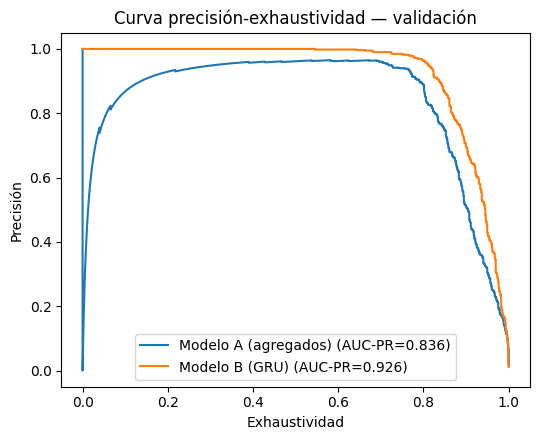
\includegraphics[width=0.62\linewidth]{informe_figuras/curva_pr_ab.png}
\end{center}

B domina a A en toda la curva precisión-exhaustividad, no solo en un punto — con la misma partición,
el mismo horizonte de predicción (por transacción) y la misma función de evaluación.

\section{Valor del orden: dos pruebas de falsificación}

Una mejora de métricas no prueba que el modelo use el orden — podría estar aprendiendo otra cosa.
Se diseñaron dos pruebas para intentar refutar esa lectura.

\textbf{Prueba 1 (obligatoria) — permutación controlada.} Se barajó el orden \emph{dentro} de cada
secuencia de prueba, sin tocar los eventos ni sus valores — la ventana contiene exactamente las
mismas transacciones, en otro orden. Se evaluó el Modelo B ya entrenado (pesos congelados) sobre
estas secuencias barajadas.

\begin{center}
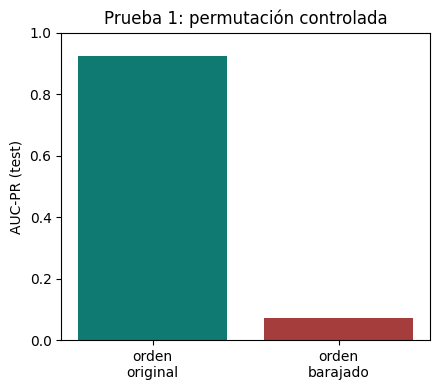
\includegraphics[width=0.4\linewidth]{informe_figuras/permutacion.png}
\end{center}

\begin{center}
\begin{tabular}{lcccc}
\toprule
 & AUC-PR & Precisión & Exhaustividad & F1 \\
\midrule
Orden original & 0.924 & 0.483 & 0.940 & 0.638 \\
Orden barajado & 0.070 & 0.132 & 0.224 & 0.166 \\
\bottomrule
\end{tabular}
\end{center}

El AUC-PR cae \textbf{92\%} al destruir el orden, con los mismos eventos. Esta es la evidencia
central: el modelo no está memorizando qué transacciones aparecen en la ventana, está leyendo la
secuencia en la que llegan.

\textbf{Prueba 2 (elegida por el equipo) — desglose por mecanismo de fraude.} De los tres tipos de
fraude generados, ``sondeo y fuga'' se diseñó para depender del orden; los otros dos, menos. Si el
razonamiento anterior es correcto, la ventaja de B debería concentrarse más en los tipos que
dependen de secuencia.

\begin{center}
\begin{tabular}{lcccc}
\toprule
Tipo de fraude & n (prueba) & Exhaustividad A / B & Puntaje prom. A & Puntaje prom. B \\
\midrule
Ráfaga alto riesgo & 183 & 0.93 / 0.93 & 0.79 & 0.90 \\
Salto de canal & 250 & 0.86 / 0.95 & 0.73 & 0.92 \\
Sondeo y fuga & 278 & 0.96 / 0.94 & 0.80 & 0.92 \\
\bottomrule
\end{tabular}
\end{center}

La exhaustividad al umbral elegido queda parecida entre A y B en los tres tipos — pero está
confundida por el umbral de A, mucho más bajo (0.05), que marca casi cualquier puntaje elevado como
fraude a costa de 827 falsos positivos en prueba (contra 714 de B). El \textbf{puntaje promedio sin
pasar por umbral} es la comparación limpia: B separa más en los tres tipos, y de forma más marcada
en salto de canal y sondeo y fuga que en ráfaga de alto riesgo — consistente con la Prueba 1, sin
exagerarla: la diferencia por tipo es real pero moderada: la evidencia fuerte de que el orden importa
sigue siendo la permutación, no este desglose.

\section{Apuesta del equipo}

\textbf{Hipótesis declarada antes de entrenar:} ``Creemos que combinar la representación secuencial
del Modelo B con las variables agregadas causales del Modelo A mejorará el AUC-PR de validación
frente al mejor de los dos por separado, porque cada rama captura una señal distinta. Lo
consideraremos útil si el AUC-PR de validación del híbrido supera al mejor de A o B en al menos
0.01.''

\textbf{Control:} mismo conjunto de entrenamiento/validación/prueba, mismo criterio de paro
anticipado, mismo `class\_weight` que B — la única diferencia es una rama adicional con los
agregados de A.

\begin{center}
\begin{tabular}{lccc}
\toprule
 & A (val.) & B (val.) & C — híbrido (val.) \\
\midrule
AUC-PR & 0.836 & 0.926 & 0.900 \\
\bottomrule
\end{tabular}
\end{center}

\textbf{Veredicto: NO ÚTIL.} El híbrido no solo no superó el margen de 0.01 exigido — quedó por
\emph{debajo} del Modelo B solo. Combinar ambas ramas no ayudó; es posible que la información de los
agregados ya esté casi contenida en lo que B aprende directamente de la secuencia cruda, y que la
rama adicional le reste capacidad de aprendizaje al resto del modelo en el mismo presupuesto de
entrenamiento. Se reporta igual, por transparencia: un resultado negativo declarado de antemano es
tan válido como uno positivo, y evita quedarnos con una arquitectura más compleja sin evidencia que
la respalde.

\section{Decisión económica}

Costo mensual estimado = (fraudes no detectados $\times$ Q4{,}200) + (transacciones legítimas
bloqueadas $\times$ Q180), con el umbral que minimiza ese costo en \textbf{validación}, aplicado una
sola vez a prueba y escalado a 30 días.

\begin{center}
\begin{tabular}{lcccc}
\toprule
Modelo & Umbral & FN & FP & Costo mensual \\
\midrule
A — agregados & 0.05 & 59 & 827 & Q440{,}733 \\
\textbf{B — secuencial} & 0.40 & \textbf{43} & \textbf{714} & \textbf{Q343{,}467} \\
C — híbrido (no recomendado) & 0.68 & 50 & 590 & Q351{,}333 \\
\midrule
Sin modelo (referencia) & — & — & — & Q3{,}318{,}000 \\
\bottomrule
\end{tabular}
\end{center}

B ahorra \textbf{Q2{,}974{,}533/mes} frente a no interceptar nada — casi Q100{,}000/mes más que A
(Q2{,}877{,}267/mes) — con \emph{menos} falsos positivos, no solo menos fraude escapado. El híbrido C
queda por encima del costo de B: no gana en AUC-PR ni en costo, así que no hay ángulo desde el que
recomendarlo sobre B.

\textbf{Límite explícito:} el punto de comparación es ``no interceptar nada'', no el motor de reglas
real del banco — no se contó con sus predicciones históricas para un contraste directo. El ahorro
reportado es frente a ese piso, no frente al sistema en producción.

\section{Recomendación y límites}

\textbf{Recomendación: complementar el sistema actual con el Modelo B secuencial}, no reemplazarlo
de golpe — el margen de mejora es consistente en AUC-PR, en las dos pruebas de falsificación y en
costo, pero el modelo no se ha probado contra el motor de reglas real ni contra tráfico en producción.

\textbf{Patrón de error concreto:} en la variante ``lenta'' de sondeo y fuga (diseñada para ser
difícil — el salto de monto es menos extremo y el episodio se extiende por horas, no minutos), el
Modelo A le asigna un puntaje promedio notablemente más bajo que al resto del fraude (0.66 contra
0.78), aunque con el umbral tan permisivo que eligió A (0.05) termina igual marcándola casi siempre.
Con un umbral más alto o más casos de este tipo, es exactamente el patrón que se le escaparía a A.

\textbf{Condiciones bajo las que cambiaría esta recomendación:} (a) si el motor de reglas real,
puesto a competir de verdad, ya cubre casos equivalentes al sondeo y fuga con un costo operativo
menor al de mantener un modelo adicional; (b) si aparece un mecanismo de fraude no visto durante el
entrenamiento y el desempeño de B se degrada más que el de A al enfrentarlo — no evaluado en este
proyecto; (c) si la latencia real de ensamblar la ventana de 10 eventos por transacción no es
compatible con el tiempo de decisión del banco.

\vspace{4pt}
\hrule
\vspace{4pt}
\small
\textbf{Matriz de evidencias}

\begin{tabular}{p{2.7cm}p{5.1cm}p{4.6cm}p{4.1cm}}
\toprule
Evidencia & Dónde aparece & Conclusión & Limitación \\
\midrule
1. Integridad de datos & Sección 1 & 3 tipos de fraude documentados, reproducible, sin fuga temporal & Datos sintéticos \\
2. Comparación A vs B & Sección 2, tabla y curva PR & B supera a A en toda la curva & Un solo horizonte de predicción \\
3. Valor del orden & Sección 3, permutación y desglose & Caída de 92\% en AUC-PR al barajar el orden & Desglose por tipo confundido por umbrales distintos \\
4. Apuesta del equipo & Sección 4 & Híbrido no útil, declarado de antemano & Un solo entrenamiento por modelo \\
5. Decisión económica & Sección 5, tabla de costos & B ahorra ~Q100k/mes más que A & Comparado contra ``no interceptar nada'', no contra reglas reales \\
6. Recomendación y límites & Sección 6 & Complementar con B, no reemplazar & Sin prueba ante fraude no visto ni en producción \\
\bottomrule
\end{tabular}

\end{document}
